\documentclass[12pt]{article}
\usepackage{fullpage,graphicx,psfrag,url}
\usepackage[small,bf]{caption}

\usepackage{amsmath}
\usepackage{amsthm}
\usepackage{amssymb}
\usepackage{verbatim}

\setlength{\captionmargin}{30pt}

\input defs.tex
\newcommand{\sign}{\mathop{\bf sign}}

\bibliographystyle{alpha}

\title{Symbolic Subdifferentiation in Python}
\author{Maurizio Cal\'o and Jaehyun Park\\
EE 364B Project Final Report\\
Stanford University, Spring 2010-11}

\begin{document}
\maketitle

\section{Introduction}
\subsection{Motivation}
Motivated by the first two weeks of lectures, we decided to create a
Python package \verb'Subgradient-PY' (\verb'SPY') that solves
optimization problems using subgradient methods. Using \verb'SPY', one can formulate and solve a convex optimization problem using the
following syntax (subject to change):

\subsection{Implementation}
Along with \verb'CVX'-like library functions, \verb'SPY' will implement three
important classes:
\begin{itemize}
\item Expression: Any real-valued mathematical expression is an object
of Expression type. It can contain variables whose values are not
predetermined.
\item Constraint: A constraint is an inequality of the form
$(\mbox{convex}) \le (\mbox{concave})$ or an equality of the form
$(\mbox{affine}) = (\mbox{affine})$.
\item (Optimization) Problem: A problem is a triplet of the form (minimize/maximize, objective, list of constraints).
\end{itemize}

The essential part of the project is to compute subgradients correctly
and efficiently, since all other methods will rely heavily on subgradients.

\section{A Quick Start}
\verb'SPY' can be downloaded from \url{http://www.stanford.edu/~liszt90/spy}. There is no installation package, so one can simply download the codes and unzip it to a directory named \verb'spy'.
\begin{verbatim}
from spy import *
x = var('x')
y = var('y')
ex = max(x + y, 2 * x - y) + square(x)
constraints = [geq(x, y), leq(norm2([x, y]), 1)]
prob = minimize(ex, constraints)
(optval, optpoint) = prob.solve()
\end{verbatim}
Printing out \verb'optval' and \verb'optpoint' gives the following:
\begin{verbatim}
-0.250040107722
{'y': -0.50654454816398864, 'x': -0.50662859414656536}
\end{verbatim}
The analytic solution is $x=y=-1/2$ with the optimal value $f^\star = -1/4$.

\section{Current Progress}
\subsection{Expression Class}
Currently, the expression class only allows scalar-valued expressions. Having matrix-valued expressions will be nice, but it is not the first priority of the project.

\subsection{Computation of Subgradients}
The recursive computation of subgradients is based on the composition rule from the class \cite{subg}. Let $f(x) = h(f_1(x), \ldots, f_k(x))$ be a function, where $h$ is nondecreasing convex function, and each $f_i$ is convex. First, we compute the values of $f_1(x), \ldots, f_k(x)$. Then, compute $c \in \partial h(f_1(x), \ldots, f_k(x))$. This results in a vector of length $k$. For each $f_i(x)$, we compute $g_i \in \partial f_i(x)$. Each $g_i$ is a vector of length $k$. Finally, we return the ``weighted sum'' $g$ of the subgradients, namely
\BEAS
g &=& c_1 g_1 + c_2 g_2 + \cdots + c_k g_k \; .
\EEAS

\section{Implementation Details}

\begin{itemize}
\item Declaring variables: \\
One can declare a variable using the following syntax.
\begin{verbatim}
x = var('x')
\end{verbatim}
The object \verb'x' is a symbolic link to the variable with the identifier string \verb,'x',.
\item Forming expressions: \\
The following line creates an expression named \verb'ex'.
\begin{verbatim}
ex = abs(x - 3) + exp(x)
\end{verbatim}
\verb'SPY' does not attempt to simplify a given expression.
\item Computing values and subgradients of expressions: \\
The following code computes the value and a subgradient at a point given by \verb'varmap'.
\begin{verbatim}
varmap = {'x': 1.5, 'y': -2}
val    = ex.get_value(varmap)
g      = ex.subgrad(varmap)
\end{verbatim}
To represent a point, users should use a dictionary rather than a list of values.
\item Specifying constraints: \\
One can use \verb'leq', \verb'eq', or \verb'geq' to construct a constraint object.
\begin{verbatim}
cons = leq(norm2([x1, x2]), y)
\end{verbatim}
At construction time, \verb'SPY' will automatically check if inequalities and equalities follow the DCP ruleset.
\item Solving an optimization problem:
\begin{verbatim}
myprob = minimize(ex, [cons1, cons2])
(optval, optpoint) = myprob.solve()
\end{verbatim}
The lines above minimizes \verb'ex' subject to two constraints \verb'cons1' and \verb'cons2' using the subgradient method. As a result, the optimal point as well as the objective value at that point will be returned. Advanced users can specify the step size rule used by the method.
\end{itemize}

\subsection{Forming an Expression}
In the current version of the \verb'SPY', one can declare a variable using the following command.
\begin{verbatim}
x = var('x')
\end{verbatim}
The meaning should be clear from the syntax; the line above declares a variable whose name is \verb'x' without a value assigned to it.

With variables, it is possible to form more complicated expressions. The following line will create an expression named \verb'ex'.
\begin{verbatim}
ex = abs(x-3)+exp(x)
\end{verbatim}
The expression above corresponds to a mathematical expression $|x-3|+e^x$. It should be noted that forming an expression does not immediately compute the value of it. All computations are done lazily; the values will be computed only when the \verb'get_value' method is called on it. Internally, the expression is stored as a tree shown in the following diagram:

\begin{center}
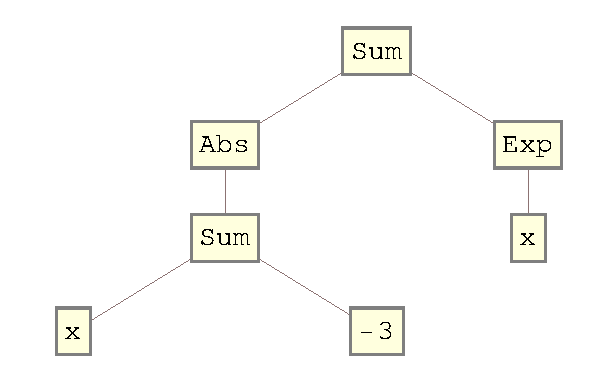
\includegraphics[width=0.45\textwidth]{expr}
\end{center}

\subsection{Retrieving Values or Subgradients}
Because the values of variables in an expression is not predetermined, a user needs to specify them manually in order to retrieve the actual value or a subgradient of the expression. The values of the variables are not passed in as a list of numbers as one might expect. Rather, the values are passed as a dictionary that maps the name of variables to their values. The benefit of this design is that one can readily access the value of a variable by its name.

\begin{verbatim}
varmap = {'x': 1.5, 'y': -2}
val    = ex.get_value(varmap)
g      = ex.subgrad(varmap)
\end{verbatim}

The code above will evaluate the expression \verb'ex' at $x=1.5$ and $y=-2$, and store the (scalar-valued) result in \verb'val'. Note that the argument to the \verb'get_value' method is a dictionary. The next line computes a subgradient of \verb'ex' evaluated at the same point, storing the result into \verb'g'. The data type of \verb'g' is the same as that of \verb'varmap'. For these methods to work correctly, users need to specify the values of all the variables present in the expression. Otherwise, \verb'nan' will be returned.

The subgradient computation, as mentioned above, is the most crucial part of this project. This feature has been tested by multiple scripts that solve simple optimization problems. Also, whenever a new library function is added, a unit test is implemented in order to ensure that the functions behave as expected.

\subsection{Library Functions}
The following list contains the functions that are implemented in the current version of \verb'SPY'. For more details, please refer to the \verb'CVX' user guide \cite{guide}.
\begin{itemize}
\item \verb'abs', \verb'max', \verb'min', \verb'pos', \verb'power', \verb'power_pos'
\item \verb'exp', \verb'log', \verb'log_sum_exp', \verb'rel_entr'
\item \verb'norm1', \verb'norm2', \verb'berhu', \verb'huber'
\item \verb'square', \verb'square_pos', \verb'sqrt', \verb'geo_mean', \verb'quad_over_lin'
\end{itemize}
Functions that take a vector as an argument (e.g. \verb'max', \verb'geom_mean') currently take a list of scalars as an input, since we don't have vector-valued expressions yet.

\section{Limitations}

\begin{itemize}
\item \verb'SPY' does not work well with equality constraints (yet).
\item Convergence behavior depends on the step sizes, so it is up to users to give a ``right'' step size rule.
\item Currently, \verb'SPY' cannot detect if the given problem is unbounded. Extending \verb'SPY' to detect unboundedness will be a great deal of work, but it will be useful.

\item Interface: To provide a clean interface to the user, we will overload operators as well as some of the Python built-in functions. This will allow users to form expressions in a more natural way. For example, \verb'abs(x - 3) + exp(x)' will give the same expression as the example shown in Section 3.1. The same principle applies to the constraint class; if an inequality or an equality has a variable in it, it will be interpreted as a constraint, rather than a boolean value.
\item Expression class: To determine whether a problem object is a valid disciplined convex optimization problem, we will implement a function that takes an expression and determines whether the function is (DCP) concave/convex. This can be done by applying the general vector composition rule \cite{cvx}, using the monotonicity and convexity properties of the atomic functions.
\item Constraint class: One important feature of the constraint class is going to be the cutting plane method. This method will return a deep cutting plane whenever a constraint is violated.
\item Problem class: We will implement both subgradient and cutting-plane methods for constrained optimization problems. The user will be able to specify which of the two methods to use, as well as the step rules.
\item Extension (tentative): After we have a basic system supporting all the features above, we will extend the code to support vectors and matrices.
\end{itemize}

\begin{thebibliography}{99}
\bibitem{subg} S. Boyd, \emph{Subgradients}, EE 364B Lecture Slides, 2011.
\bibitem{guide} M. Grant and S. Boyd, \verb'cvx' \emph{Users' Guide}, 2011.
\bibitem{cvx} S. Boyd, \emph{Convex Functions}, EE 364A Lecture Slides, 2011.
\end{thebibliography}

\end{document}
